\subsection{Configurations} \label{subsec:ConfigL2}

All the $k$-List algorithms make use of the fact that there are many solution-tuples and we are allowed to output a fraction of all the solutions. 
The main challenge in designing an efficient $k$-List algorithm is to identify a criterion s.t.\ (1) a solution that matches the criterion is easy to find, and (2) enough solutions satisfy this criterion.  The first property leads to a faster algorithm, the second is specified by the problem. In the case of the approximate $k$-List problem, we want to output almost all solutions.

To define the criterion we use in our algorithm, recall the definition of a Gram matrix.

\begin{definition}[Gram Matrix]
 For vectors $\xvec_1, \ldots, \xvec_k$ from $\R^n$, the \emph{Gram matrix} $C \in \R^{k \times k}$ is a positive semidefinite matrix whose entries are pairwise inner products: $C_{i, j} = \ScProd{x_i}{x_j}$.
\end{definition}  

Note that the Gram matrix is invariant under simultaneous rotations and reflections of all $\xvec_i$'s. This property also holds for a $k$-tuple from $\Sphere{n}$ that forms a solution to the approximate $k$-List problem as both, rotation and reflection, preserve distance. Hence, we are interested in solutions up to such symmetry. We set our searching criteria to be a specific Gram matrix of vectors $\xvec_1, \ldots, \xvec_k$ which we call a \emph{configuration}. 

\begin{definition}[Configuration] \label{def:Configuration}
	The \emph{configuration} $C = \Conf(\xvec_1, \ldots, \xvec_k)$ for $\xvec_1, \ldots, \xvec_k \in \Sphere{n}$ is the Gram matrix $C_{i, j} = \ScProd{x_i}{x_j}$.
\end{definition}

The configuration gives all the necessary information on the geometry of the tuple, and in particular
\begin{equation} \label{eq:LengthOfSum}
 \| \sum_i \xvec_i \|^2 = \sum_i \| \xvec_i \|^2 + \sum_{i \neq j} \ScProd{\xvec_i}{\xvec_j} = k + 2 \sum_{i<j}\ScProd{\xvec_i}{\xvec_j}.
\end{equation}

Let us define the space of all possible configurations for $\xvec_i \in \Sphere{n}$ together with the space of those configurations that give a tuple with the property $\| \sum_i \xvec_i \|^2 \leq t$:
\begin{align*}
	&\ConfSpace = \{ C \in \R^{k \times k} \; |  \; C \text{ symmetric positive semi-definite}, C_{i,i}=1 \}, \\
	&\ConfSpacet = \{ C \in \ConfSpace \; | \; \sum_{i,j} C_{i,j} \leq t^2 \}.
\end{align*}

For fixed $k$, we think of the set $\ConfSpace$ as a finite set which we can efficiently enumerate.  
Observing that a tuple $(\xvec_1, \ldots, \xvec_k)$ is a solution to the approximate $k$-List problem iff $\Conf(\xvec_1, \ldots, \xvec_k) \in \ConfSpacet$, immediately gives us an algorithm: we enumerate over all configurations in $\ConfSpacet$ and solve the \emph{$k$-List configuration problem} defined as follows.

\begin{definition}[Configuration Problem] \label{def:ConfigProblem}
Given $k$ exponentially sized lists $L_1, \ldots, L_k$ of vectors from $\Sphere{n}$, a target configuration $C \in \ConfSpace$, and $\eps>0$, the task is to output \emph{all} $k$-tuples $\xvec_1 \in L_1, \ldots, \xvec_k \in L_k$ s.t.\ $| \ScProd{\xvec_i}{\xvec_j} - C_{i,j}| \leq \eps$ for all $i, j$. Such a tuple is called a solution to the Configuration problem.
\end{definition}

\begin{remark}
To simplify the analysis, we assume we can compute with real numbers. Our algorithm and the analysis remain true when we use sufficiently precise approximations. Since the inner products $\ScProd{\xvec_i}{\xvec_j}$ take real values, asking for the exact equality to $C$ does not bring any solution. We, therefore, introduce some small $\eps > 0$. For two configurations $C, C'$, we write $C \approx_{\eps} C'$ when $| C_{i,j} - C'_{i,j} | \leq \eps$. 
\end{remark}

The crucial property of a solution $(\xvec_1, \ldots, \xvec_k)$ to the Configuration problem is the fact that it can be \emph{locally} verified as we only have to look at \emph{pairs} $\xvec_i, \xvec_j$. Note that a solution to the approximate $k$-List problem as given in Def.~\ref{def:kListL2} does not share this `locality' feature. 

Now we have an algorithm to solve the $k$-List problem: (1) enumerate all the configurations $C \in \ConfSpacet$, and (2) solve the Configuration problem for each $C$. Below we show how to bypass the first step. It turns out that we do not have to enumerate all the configurations to output a $1-\smallo(1)$-fraction of the solutions to the $k$-List problem. There exist one particular configuration, later denoted as $\Cbalt$, which is attained by most of the solutions. This allows us to solve the Configuration problem only for $\Cbalt$ to obtain enough solution-tuples for the $k$-List problem. To give $\Cbalt$ explicitly, we study the Wishart distribution \cite{Wishart28}, which is a matrix generalization of the chi-squared distribution.

\paragraph{Wishart distribution.} Consider $k$ vectors $\xvec_1, \ldots, \xvec_k \in \R^{n+1}$ sampled independently from $(n+1)-$ dimensional spherical Gaussian (mean $0$ and standard deviation\ $1$). Set $S_{i,j} = \ScProd{\xvec_i}{\xvec_j} \in \R^{k \times k}$. For integer $k, n$ with $n+1 > k-1$, a random $k \times k$ symmetric matrix $S$ has a Wishart distribution with the probability density function
\begin{equation} \label{eq:WishartDensity}
	\pW(S) = \frac{e^{-\tfrac{1}{2} \cdot \Tr S} \cdot \det(S)^{\frac{n-k}{2}}}{2^{\frac{(n+1)k}{2}} \pi^{\frac{k (k-1)}{4}} \prod_{i=0}^{k-1} \Gamma \bigl( \frac{n+1-i}{2} \bigr)}  \d S,
\end{equation}
where $\d S = \prod_{i \leq j} \d S_{i,j}$, $\Gamma(z) = \int\limits_0^\infty x^{z-1} e^{-x}\d x$ is the Gamma-function, and $\Tr(S)$ is the trace-function (i.e., the sum of the main-diagonal elements of $S$). A derivation of these density can be found in \cite{Eaton07}. 

Note that matrix $S$ is a Gram matrix of vectors \emph{not} from $\Sphere{n}$. To get the density function for distribution on our configuration space $\ConfSpace$ where vectors are sampled uniformly from the $n$-sphere, we have to normalize $S$ and change the reference density $\d S$ appropriately. 

\begin{thm} \label{thm:WishartDist}
Let $\xvec_1, \ldots, \xvec_k \in \Sphere{n}$ be independent uniformly distributed on the $n$-sphere, $n > k$. Then the configuration $C = \Conf(\xvec_1, \ldots, \xvec_k)$ follows a distribution $\pC$ on $\ConfSpace$ with the probability density function
\[
	\pC (C) = W_{n,k} \cdot \det(C)^{\tfrac{1}{2}(n-k)} \d \ConfSpace = \softO_k \Bigl( \det(C)^{\tfrac{n}{2}}\Bigr) \d \ConfSpace,
\]
where $\d \ConfSpace = \d C_{1,2} \cdots \d C_{k-1, k}$ and $W_{n,k} = \pi^{-\frac{k(k-1)}{4}} \prod_{i=0}^{k-1} \frac{\Gamma \bigl( \frac{n+1}{2} \bigr)}{\Gamma\bigl( \frac{n+1-i}{2} \bigr)} = \softO_k\Bigl( n^{\frac{(k-1)k}{4}} \Bigr)$ is a normalization constant that only depends on $n$ and $k$.
\end{thm}

\begin{proof}
	Let $C_{i,j} = \frac{S_{i,j}}{\sqrt{S_{i,i} S_{j,j}}}$, where $S$ follows the Wishart distribution with pdf given in Eq.~(\ref{eq:WishartDensity}). This normalization defines the map $\Phi$ from $\R^{\frac{k(k+1)}{2}}$ to itself that represents the following change of variables:
	\begin{align*}
		\Phi&(S_{1,1}, S_{2,2}, \ldots, S_{k,k}, S_{1,2}, \ldots, S_{1,k}, S_{2,3}, \ldots, S_{k-1, k}) = \\
		&(S_{1,1}, S_{2,2}, \ldots, S_{k,k}, \tfrac{S_{1,2}}{\sqrt{S_{1,1} S_{2,2}}}, \ldots, \tfrac{S_{1,k}}{\sqrt{S_{1,1} S_{k,k}}}, \tfrac{S_{2,3}}{\sqrt{S_{2,2} S_{3,3}}}, \ldots, \tfrac{S_{k-1,k}}{\sqrt{S_{k-1,k-1} S_{k,k}}}) = \\
		&(S_{1,1}, S_{2,2}, \ldots, S_{k,k}, C_{1,2}, \ldots, C_{1, k}, C_{2,3}, \ldots, C_{k-1, k}).
	\end{align*}
	Note that we keep the diagonal elements $S_{i,i}$ to make the transformation $\Phi$ injective, as we want to apply the substitution rule $\prod_{i=1}^k \d S_{i,i} \prod_{i <j} C_{i,j} = | \det (D \Phi) | \cdot \prod_{i \leq j} \d A_{i,j}$, where $D \Phi$ is the Jacobian of $\Phi$. This Jacobian is a triangular matrix with the main diagonal 
	\[(1, \ldots, 1, \frac{1}{\sqrt{S_{1,1} S_{2,2}}}, \ldots, \frac{1}{\sqrt{S_{1,1} S_{k,k}}}, \frac{1}{\sqrt{S_{2,2} S_{3,3}}}, \ldots, \frac{1}{\sqrt{S_{k-1,k-1} S_{k,k}}}),  
	\]
	so its determinant is $|\det (D \Phi)|  = \prod_i \frac{1}{\sqrt{S_{i,i}}^{k-1}}$.
	Further, we can express $S$ as $S = T C T$, where $T$ is a diagonal matrix with $(\sqrt{S_{1,1}}, \ldots, \sqrt{S_{k,k}})$ on the main diagonal. Therefore, $\det(S) = \det(C) \cdot \prod_i S_{i,i}$. Applying the transformation to the Wishart density function, one readily obtains a pdf.\ in $(S_{1,1}, \ldots, S_{k,k}, C_{1,2}, \ldots, C_{k-1,k})$-variables
	\begin{equation} \label{eq:rhoWishProof}
		\pW = \frac{ e^{-\frac12\sum_i S_{i,i}} \det(C)^{\frac{n-k}{2}} \prod_i S_{i,i}^{\frac{n-k}{2}}}{2^{\frac{(n+1)k}{2}} \pi^{\frac{k(k-1)}{4}} \prod_{i=0}^{k-1} \Gamma(\frac{n-i+1}{2} ) } \prod_i\sqrt{S_{i,i}}^{k-1}\prod_i \d S_{i,i}\prod_{i<j}\d C_{i,j}.
	\end{equation}
	As we want to relate the distribution to $C_{i,j}$ only, we integrate over $\prod_i \d S_{i,i}$ to obtain the desired $\pC$. From Eq.~(\ref{eq:rhoWishProof}), it follows that $\pC$ is of the form $\pW = W_{n,k} \det(C)^{\frac{n-k}{2}} \d \ConfSpace$ for some factor $W_{n,k}$ that depends only on $k$ and $n$. We write $W_{n,k}$ as $W_{n,k} = \frac{1}{t} e^{-\frac12\sum_i S_{i,i}} \prod_i S_{i,i}^{\frac{n-k}{2}}$, where $t$ is the denominator in Eq.~(\ref{eq:rhoWishProof}), and compute
	\begin{align*}
		W_{n,k} &= \frac{1}{t} \idotsint\limits_{A_{1,1}\hspace{1.3em}A_{k,k}} e^{-\frac12\sum_i S_{i,i}} \prod_i S_{i,i}^{\frac{n-k}{2}} \prod_i\sqrt{S_{i,i}}^{k-1}\prod_i \d S_{i,i} \\
		&=\frac{1}{t} \idotsint\limits_{A_{1,1}\hspace{1.3em}A_{k,k}}e^{-\frac12\sum_i S_{i,i}} \prod_i S_{i,i}^{\frac{n-1}{2}}\prod_i \d S_{i,i} \\
		&=\frac{1}{t} \Bigl( \int\limits_{S_{1,1}=0}^{+ \infty} S_{1,1}^{\frac{n-1}{2}} e^{-\frac12 S_{1,1}} \d S_{1,1}\Bigr)^k \\
		&=\frac{2^{\frac{k(n+1)}{2}}}{t} \Bigl( \int\limits_{S_{1,1}=0}^{+ \infty} \Bigl( \frac{S_{1,1}}{2} \Bigr)^{\frac{n+1}{2} - 1} e^{-\frac12 S_{1,1}} \d \frac{S_{1,1}}{2}\Bigr)^k \\
		&=\frac{2^{\frac{k(n+1)}{2}}}{t} \Bigl( \int\limits_{x=0}^{+ \infty} x^{\frac{n+1}{2}-1} e^{-x} \d x \Bigr)^k \\
		&=\frac{2^{\frac{k(n+1)}{2}} \cdot \Gamma \Bigl( \frac{n+1}{2} \Bigr)^k}{t}
		=\frac{\Gamma \bigl( \frac{n+1}{2} \bigr)^k}{\pi^{\frac{k(k-1)}{4}} \prod_{i=0}^{k-1} \Gamma(\frac{n-i+1}{2} )}.
	\end{align*}
	From Stirling's formula, $\Gamma(n) \sim \bigl( \tfrac{n}{e} \bigr)^n$, we have for any fixed $z$ and $n \rightarrow \infty$, $\frac{\Gamma(n+z)}{\Gamma(n)} = \bigO_z(n^z)$. Finally, we have
	\[
		W_{n,k} = \bigO_k \Bigl( n^{\sum_{i=0}^{k-1} \tfrac{i}{2}}\Bigr) = \bigO_k \Bigl( n^{\frac{k(k-1)}{4}} \Bigr).
	\]
\end{proof}

Since we now know the distribution on the space $\ConfSpace$, we want to find a configuration $C \in \ConfSpace$ with the largest mass. It turns out that this is a configuration with the highest amount of symmetry, i.e.\ when all off-diagonal entries are equal. We prove this statement in Thm.~\ref{thm:maxConfig} below. We call such configurations \emph{balanced} and denote them $\Cbal$.

\begin{definition}[Balanced Configuration] \label{def:BalancedConfig}
 A configuration $\Cbal \in \ConfSpace$ is balanced if $C_{i,j} = C_{i', j'}$ for all $i \neq i', j \neq j'$. A balanced configuration that additionally belongs to $\ConfSpacet$ for some target length $t>0$ is denoted $\Cbalt$.
\end{definition} 

Before showing that $\pC$ indeed attains its maximum at $\Cbal$, we compute the determinant of $\Cbal$.
\begin{lemma} \label{lem:CBalancedDet}
\text{Let }
\begin{align*}
C = \begin{psmallmatrix}
         1 & a & a &\ldots & a\\
         a & 1 & a &\ldots & a\\
         a & a & 1 &\ldots & a\\
         & \vdots& &\ddots & \vdots\\
         a & a & a &\ldots & 1
         \end{psmallmatrix}\in\R^{k\times k}.
\end{align*}
Then $\det(C) = (1-a)^{k-1}(1+(k-1)a)$.
\end{lemma}
\begin{proof}
	We write $C = (1-a) \cdot \Id_k + a \cdot \onevec \cdot \onevec^t$. Sylvester's Determinant Identity states that $\det(\Id_m + AB) = \det(\Id_n + BA)$ for any $A$ and $B$ of dimensions $m \times n$ resp.\ $n \times m$. It follows that
	\begin{align*}
	\det(C) &=  \det \bigl( (1-a) (\Id_k + \tfrac{a}{a-1} \onevec \cdot \onevec^t) \bigr) = (1-a)^k \det \bigl( \Id_1 + \tfrac{a}{a-1} \onevec^t \cdot \onevec \bigr) \\
	&=(1-a)^k \bigl( 1 + \tfrac{a}{1-a}k \bigr) = (1-a)^{k-1} (1+(k-1)a).
	\end{align*}  
\end{proof}

The space of all configurations $\ConfSpace$ is compact\footnote{Closeness immediately follows from the fact that $\ConfSpace \subset \R^{k^2}$; further, all entries of an element from $\ConfSpace$ are bounded, in particular, $C_{i,j}\leq 1$.} and, therefore, integrating over it will asymptotically pick the maximum value. So the probability that a uniform random tuple $(\xvec_1, \ldots, \xvec_k)$ forms a  ``good'' configuration from $\ConfSpacet$, and consequently, gives a solution to the Configuration problem, is
\[
 \int\limits_{\ConfSpacet} \pC = \softO(\max\limits_{C \in \ConfSpacet} \det(C)^{n/2}).
\]

The next theorem determines this maximum.

\begin{thm} \label{thm:maxConfig}
	Let $0 < t < \sqrt{k}$ be a target length and $\ConfSpacet \subset \ConfSpace$ be the subset of configurations with target length at most $t$. Then $\det(C)$ attains its unique maximum over $\ConfSpacet$ at the balanced configuration $\Cbalt$ with $C_{i,j} = \frac{t^2-k}{k^2-k}$ for all $i \neq j$ with maximal value
	\[
		\det(\Cbalt) = \frac{t^2}{k} \left( \frac{k^2-t^2}{k^2-k} \right)^{k-1}.
	\] 
	In particular, for $t=1$, $C_{i,j} = -\frac{1}{k}$ and $\det(\CbalOne) = \frac{(k+1)^{k-1}}{k^k}$.
\end{thm}

\begin{proof}
	For $k=2$, the statement immediately follows from Eq.~(\ref{eq:LengthOfSum}). So assume $k \geq 3$. 
	
	Consider configurations $C$ with $\Tr(C) = k$ and $\sum_{i,j} C_{i,j} \leq t^2$. This is clearly weaker than the condition $C_{i,i}=1$ and later we show that the stronger condition is met at the maximum.
	
	From the fact that $C$ is a Gram matrix, and hence, it is positive semi-definite, it follows that its eigenvectors $\vvec_1, \ldots, \vvec_k$ form an orthonormal basis and its eigenvalues $0 \leq \lambda_1 \leq \ldots \leq \lambda_k$ are positive. 
	
	We have $\Tr(C) = \sum_i \lambda_i$ and $\det(C) = \prod_i(\lambda_i)$. We want to find $\lambda_i$'s that maximize the determinant. In particular, we show that $\onevec$ is an eigenvector for maximal $\det(C)$. To see this, write $\sum_{i,j} C_{i,j}  = \onevec C \onevec\transpose$, so for the smallest eigenvalue $\lambda_1$ it holds
	\begin{equation} \label{eq:SmallestEigenvalue}
		t^2 \geq \onevec C \onevec\transpose \geq \lambda_1 \| \onevec \|^2 = k \lambda_1.
	\end{equation}
	We have $\lambda_1 \leq \tfrac{t^2}{k} < 1$. The Arithmetic Mean-Geometric Mean inequality stating that for non-negative real $x_i$'s, $ \tfrac{\sum_i x_i}{n} \geq \sqrt[n]{\prod_i x_i}$, gives for $\det(C) = \lambda_1 \prod_{i=2}^k \lambda_i$ and $\sum_{i=2}^k \lambda_i = k - \lambda_1$:
	\[
			\det(C) \leq \lambda_1 \left( \frac{k-\lambda_1}{k-1} \right)^{k-1}.
	\]
	As the derivative of the right-hand side w.r.t.\ $\lambda_1$, $ \tfrac{k(1-\lambda_1)}{k-1} \bigl( \tfrac{k-\lambda_1}{k-1} \bigr) ^{k-2} > 0$, is everywhere positive, we bound $\det(C)$ by plugging in the maximal $\lambda_1 = \tfrac{t^2}{k}$:
	\begin{equation} \label{eq:IneqForDetC}
		\det(C) \leq \lambda_1 \left( \frac{k-\lambda_1}{k-1} \right)^{k-1} \leq \frac{t^2}{k} \left( \frac{k - \tfrac{t^2}{k}}{k-1}\right)^{k-1} = \frac{t^2}{k} \left( \frac{k^2 - t^2}{k^2-k}\right)^{k-1}.
	\end{equation}
	The first inequality in Eq.~(\ref{eq:IneqForDetC}) becomes an equality iff $\lambda_2 = \ldots = \lambda_k$ and the second  when $\lambda_1  = \tfrac{t^2}{k}$. In this case, from $\Tr(C) = k$, we have $\lambda_2 = \tfrac{k^2-t^2}{k(k-1)}$ and $\onevec$ is an eigenvector of $C$ with eigenvalue $\lambda_1$. 
	
	Now we show that $C_{i,i} = 1$ for maximal $\det(C)$ and $C_{i,j}$ for $i \neq j$ as in the theorem statement. Consider the eigendecomposition $C = V \Lambda V^{-1} = V \Lambda V\transpose$, where $V$ is the orthonormal matrix with $\vvec_i$'s as columns, $\Lambda$ is the diagonal matrix with $\lambda_i$'s on the main diagonal. Equivalently, we can write
	\[
		C = \sum_i \lambda_i \vvec_i \vvec\transpose_i  = (\lambda_1 - \lambda_2) \vvec_1 \vvec\transpose_1 + \lambda_2 \sum\limits_{i=1}^k \vvec_i \vvec\transpose_i = \frac{\lambda_1 - \lambda_2}{k} \onevec \onevec\transpose + \lambda_2 \Id_k.
	\]
	Therefore, all the diagonal entries of $C$ are equal to $\tfrac{\lambda_1 - \lambda_2}{k} + \lambda_2$ and all the off-diagonal entries are equal to $\frac{\lambda_1 - \lambda_2}{k}$. The theorem follows once we substitute the eigenvalues $\lambda_1 = \tfrac{t^2}{k}$, $\lambda_2 = \tfrac{k^2 - t^2}{k(k-1)}$ for maximal $\det(C)$.
\end{proof}

In case we search for configurations with the target length $t > \sqrt{k}$, the proof should consider the largest eigenvalue $\lambda_k$ instead of the smallest $\lambda_1$.

Also from the above proof it follows that looking at `only-1' linear combination of $\xvec_i$'s is optimal. If instead we look for $\| \sum_i a_i \xvec_i \| \leq t$ for some $\avec \neq \onevec$, the set of `good' configurations $\ConfSpacet$ would be $\{ C \in \ConfSpace \; | \; \| \avec\transpose C \avec \| \leq t  \}$ and in the proof above the eigenvector $\onevec$ would be replaced by $\avec$. Since $\onevec$ has the minimal norm, the configurations from $\ConfSpacet$ we are looking at are optimal.

In case $t=1$, the balanced configuration $(\xvec_1, \ldots, \xvec_k)$ forms a regular $k+1$-dimensional simplex with center in the origin (the condition on pair-wise inner products $\ScProd{\xvec_i}{\xvec_j} = -\tfrac{1}{k}$ matches with the central angle for the regular simplex). The missing $k+1\st$ point of the simplex is $-\sum_i \xvec_i$, i.e.\ the negative of the sum (see Fig.~\ref{fig:Tetrahedron}).

From our concentration result, it follows that a random $k$-tuple from $\Sphere{n}$ is a solution to the Configuration problem with probability $\softO( \det(\Cbalt)^{n/2})$. Since we know the size of input list $L_i$, we can compute the expected number of solutions.

\begin{figure}[t]
	\centering
	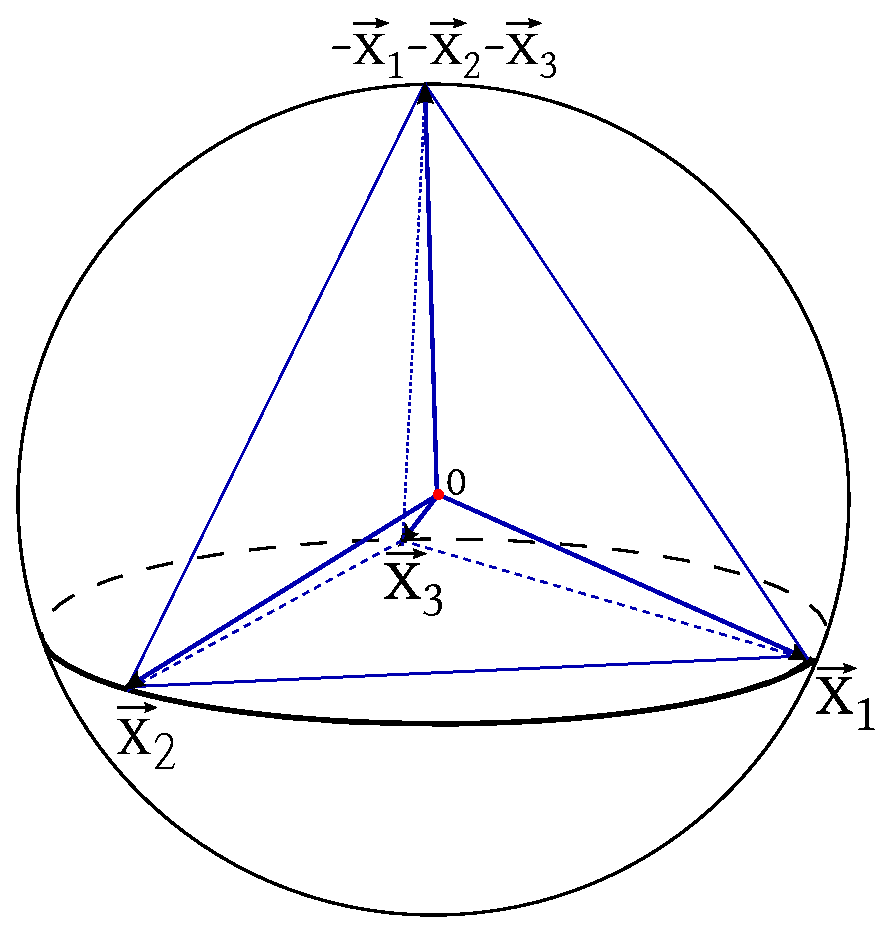
\includegraphics[scale=0.38]{tetrahedron}
	\caption[Balanced Configuration]{A regular tetrahedron ($3-$simplex) represents a balanced configuration for $k=3$.}
	\label{fig:Tetrahedron}
\end{figure}

\begin{corollary} \label{cor:NumberOfSolutions}
	Let $k,t$ be fixed. Then the expected number of solutions to the Configuration problem with input lists of size $|L|$ is
	\begin{equation} \label{eq:ExpNumberOfSolutions}
	\E[\# \text{solutions}] = \softO \left( |L|^k \Bigl(\frac{t^2}{k} \Bigl( \frac{k^2-t^2}{k^2-k} \Bigr)^{k-1}  \Bigr)^{\tfrac{n}{2}} \right).
	\end{equation}
\end{corollary}
\begin{proof}
	The total number of $k$-tuples is $|L|^k$. From Thms.~\ref{thm:WishartDist} and \ref{thm:maxConfig}, the probability that a random $k$-tuple forms a configuration from $\ConfSpacet$ is $\softO( \det(\Cbalt)^{n/2})$. Thm.~\ref{thm:maxConfig} states the value for this determinant.
\end{proof}

As a consequence, we can easily compute the size of input lists for a desired output list's size. In algorithms for \SVP, $t=1$ and the output list is required to have the same size as input lists. The following corollary proves the conjecture stated in \cite{BLS16}.

\begin{corollary} \label{cor:BalancedListSizes}
Let $k$ be fixed and $t=1$. In the Configuration problem, for the input lists each of size $|L|$, the output list is expected to be of size $|L|$ if $|L|  = \softO \Bigl( \Bigl( \frac{k^{\tfrac{k}{k-1}}}{k+1} \Bigr)^{\tfrac{n}{2}} \Bigr)$. 
\end{corollary}
\begin{proof}
	The statement immediately follows from setting the expression in Eq.~(\ref{eq:ExpNumberOfSolutions}) equal to $|L|$ for $t=1$. 
\end{proof}

Finally, we argue that solving the Configuration Problem gives a $1-\smallo(1)$ fraction of solutions for the $k$-List problem. This follows from Thm.~\ref{thm:maxConfig}. Essentially it states that for any fixed $\eps>0$, the probability that a randomly chosen solution to the approximate $k$-List problem forms a configuration $\eps$-close to $\Cbalt$, converges exponentially to $1$ as $n \rightarrow \infty$. Therefore, solving the $k$-List Configuration problem for $\CbalOne$ and restricting to only those solutions whose sum is at most $t$, gives a $1-\smallo(1)$ fraction of solutions for the approximate $k$-List problem. These arguments justify the following corollary.

\begin{corollary}\label{cor:ReductionToConfigProblem}
Let $k,t$ be fixed. Then the approximate $k$-List problem with target length $t$ can be solved in the same time as the $k$-List configuration problem with target configuration $\Cbalt$ for any fixed $\eps>0$.
\end{corollary}